\subsection{Follow me cloud} \label{fmc}

Asiakaslaitteiden määrän kasvu sekä tietoliikenne-intensiivisien sovelluksien käytön yleistyminen aiheuttaa suurta kuormaa verkkoinfrastruktuurille \cite{taleb2013follow}. Ongelmat johtuvat pääasiassa mobiiliverkon keskitetystä rakenteesta, jossa tietoliikenneyhteydet kerätään kulkemaan keskitetyn pisteen kautta \cite{taleb2013follow}. Tämän lisäksi yhteyksissä on huomattavasti viivettä, koska asiakkaan ja palvelimen väliset yhteydet ovat pitkiä. Follow me cloud (FMC) ehdottaa ratkaisua, jossa operaattorin keskitetty verkkorakenne muutettaisiin hajautetuksi \cite{taleb2013follow}.
Käytännössä tämä tarkoittaisi, että EPC:n ja ulkoverkon välisten yhdyskäytävien, eli P-GW instanssien, määrää lisättäisiin. 
Toinen osa ideaa on, että P-GW:t voitaisiin hajauttaa palvelinsaleihin lähemmäksi asiakkaan käyttämiä palveluita. Tämä siksi, että myös mobiiliverkkojen operaattorit ovat huomanneet hajautustarpeen ja alkaneet hajauttaa mobiiliverkkoja \cite{taleb2013follow}. 
FMC:n arkkitehtuuri edellyttää hajautettua EPC:tä ja hajautettuja palvelinkeskuksia. 

Asiakaslaitteen yhdistäessä verkkoon, verkkoyhteyksien kiintopisteenä toimii todennäköisimmin lähimpänä sijaitseva P-GW. 
Perinteisessä mobiiliverkossa keskitetystä rakenteesta johtuen, asiakaslaite pysyy yhden P-GW:n asiakkaana, vaikka liikkuisi mobiiliverkossa.
FMC lähteekin ratkaisemaan ongelmaa jossa asiakaslaitteelle tarjottaisiin aina optimaalisin\footnote{optimaalisella tarkoitetaan tässä yhteydessä parasta mahdollista, käyttäen mittareina fyysistä sijaintia ja kuormaa} yhteys tavoiteltuun palveluun.

FMC:n ratkaisemat ongelmat voidaan jakaa kahteen osaan: optimaalisen reitin valitseminen ja optimaalisen reitin ylläpitämiseen käyttäjän liikkuessa. 
Reitinvalinta jakautuu matkaan, jonka asiakkaan yhteys kulkee mobiiliverkossa, eli tarkemmin ottaen EPC:n sisällä, sekä matkaan P-GW:ltä kohdepalvelimeen. Tämän saavuttamiseksi mobiiliverkon arkkitehtuurin tarvitaan palvelinkeskuksien ja P-GW välisiä mappauksia tekevä entiteetti. 

\begin{figure}[tb]
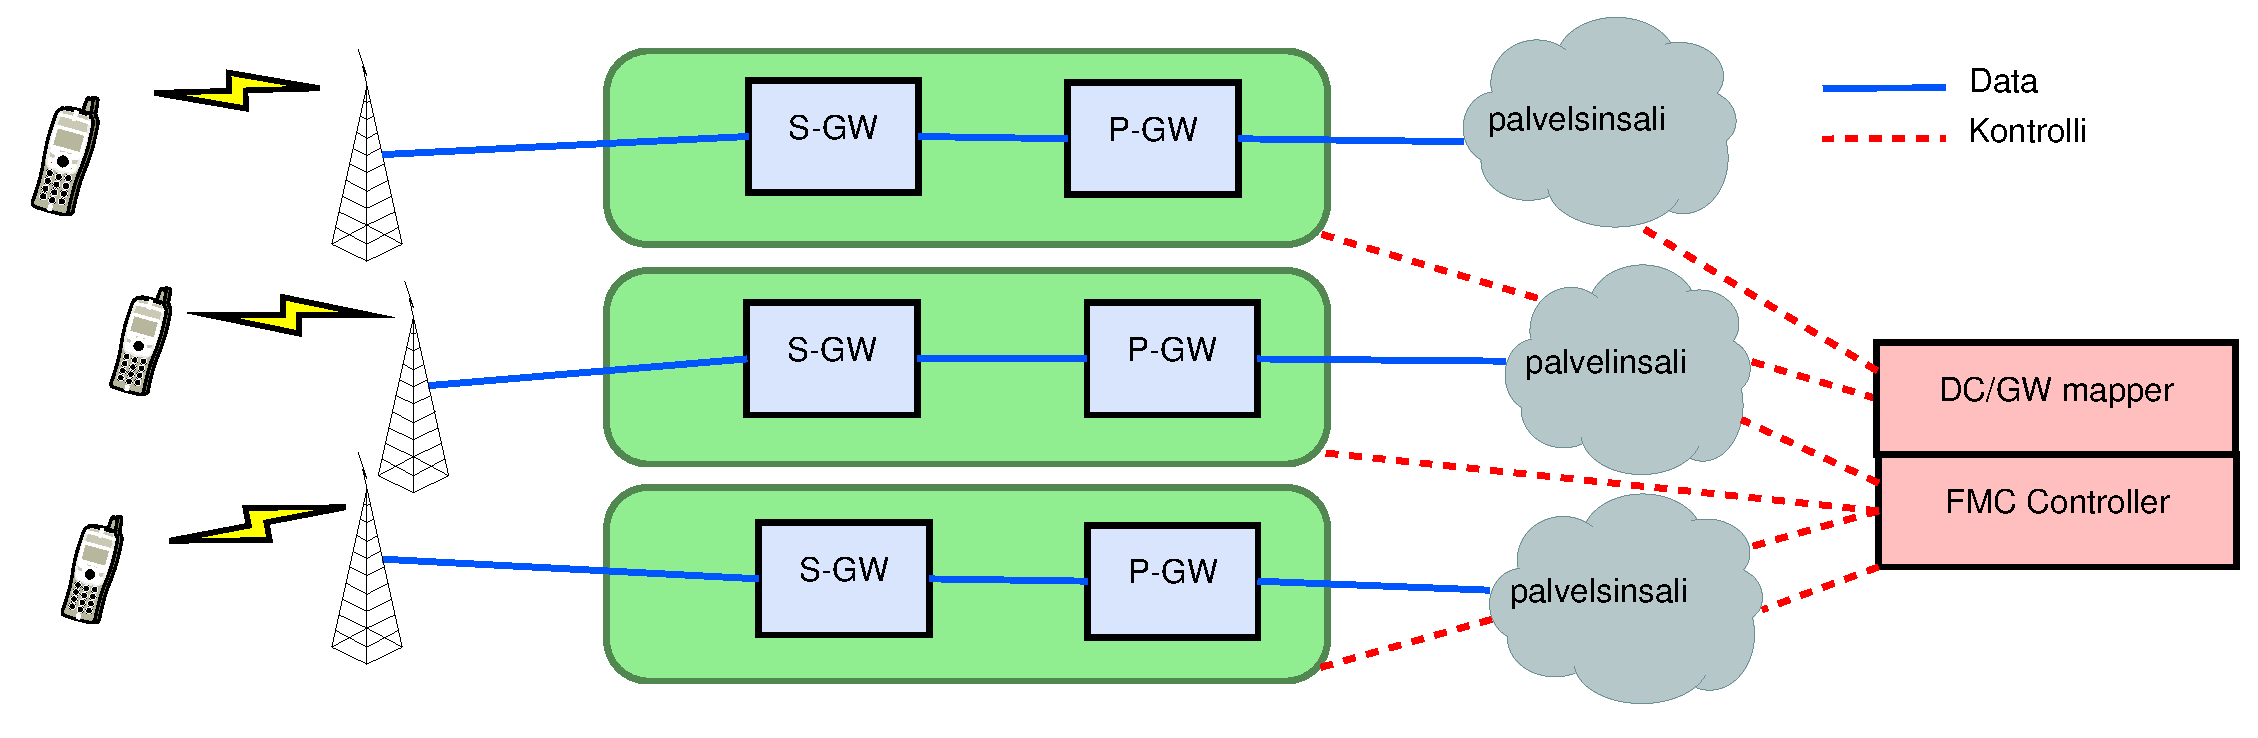
\includegraphics[width = \textwidth]{FMC.eps}
\caption{Follow me cloud arkkitehtuuri, jossa mobiiliverkko on hajautettu useampaan yhdyskäytävään. Mukaelma artikkelissa \cite{mach17mobile} esitetystä kuvasta} \label{fig:fmc}
\end{figure}

FMC tarjoaa optimaalisen reitin löytämiseen ratkaisua, jossa mobiiliverkon läheisyyteen lisättäisiin hallinnolliset entiteetit FMC controller ja DC/GW mapper.
Lisäksi ehdotuksessa mobiiliverkkoon lisätään tunnisteet, joiden avulla asiakaslaitteen sijainti saadaan selville asiakaslaitteen käyttämästä yhteydestä.
DC/GW mapper tehtävä on valita asiakkaan yhteyttä parhaiten vastaava palvelinsali.
DC/GW mapperin paritus tehdään esimerkiksi yhdistämällä tietyn P-GW:n (voidaan päätellä esimerkiksi IP-vyöhykkeen avulla) kautta tulevat yhteydet ennalta määrättyyn palvelinsaliin. 
Kuvassa \ref{fig:fmc} asiakaslaitteet ovat yhdistyneenä oman S-GW/P-GW-parin kautta, kyseistä yhdyskäytävää vastaavaan palvelinsaliin. 

Toinen osa ratkaisua on asiakaslaite–palvelinsali-yhteyden ylläpitäminen.
Yhteyden ylläpitäminen asiakkaan liikkuessa vaatii jonkin verran muutoksia tapaan, jolla käyttäjän siirtymiseen mobiiliverkossa reagoidaan. 
Hajautetussa mobiiliverkossa tutkiaseman vaihtuessa, myös tietoliikenne yhteyskäytävänä toimiva P-GW saattaa vaihtua.
Tämän seurauksena asiakaslaitteen IP-osoite vaihtuu ja yhteys reunapalveluun katkeaa.
FMC on esittänyt, että asiakas ja reunapalvelu yhdistettäisiin erillisen tunnisteen perusteella, joka generoidaan asiakastunnisteen ja palvelutunnisteen pohjalta.
Tämä uusi tunniste korvaa IP-osoitteet ja mahdollistaan yhteyksien uudelleenmuodostuksen tilanteissa, joissa asiakaslaitteen tai reunapalvelun IP-osoitteet vaihtuvat.

FMC controllerin tehtävänä on laukaista palvelun siirtäminen optimaalisempaan palvelinsaliin esimerkiksi asiakaslaitteen yhteysmuutoksien seurauksena.
FMC controller tekee päättelyä siitä kannattaako reunapalvelua siirtää.

FMC eroaa muista mobiiliverkon ratkaisuista sillä, että se ei tuo palvelinresursseja osaksi mobiiliverkkoa. Lisäksi FMC ei tee mobiiliverkon toiminnallisuuksiin muutoksia. FMC pyrkii takaamaan nopeimman mahdollisen yhteyden haluttuun palveluun. FMC jättääkin auki mahdollisuuden, että reunapalvelut tarjoaa joku muu kuin mobiiliverkon operaattori.
Koska reunapalvelimet sijaitsevat mobiiliverkon ulkopuolella FMC ei edellytä muutoksia myöskään mobiiliverkon sisäiseen reititykseen.
